\documentclass[a4paper,12pt]{article}
\usepackage[english]{babel} 
%\usepackage[italian]{babel} 
%\usepackage[latin1]{inputenc} 
\usepackage[dvips]{graphicx}
\usepackage{amssymb}
\usepackage[width=125mm]{caption}
\usepackage{amsthm}
\usepackage[ND,SEQ]{prftree}
\usepackage{mathrsfs}
\usepackage{graphicx}
\usepackage{amsmath}


\usepackage{fancyhdr}
 
\pagestyle{fancy}
\fancyhf{}
%\fancyhead[CE]{\leftmark}
\fancyhead[CO]{\rightmark}
\fancyfoot[CE,CO]{\thepage} 
\renewcommand{\headrulewidth}{1pt}
%\renewcommand{\footrulewidth}{1pt}   %not visible if commented 

\usepackage[pdfauthor={Paolo Comensoli},
pdftitle={Applications of hyper-resolution, 
Paolo Comensoli}, pagebackref=false,bookmarksopen=true]{hyperref}
% pagebackref: se vero, ad ogni voce di bibliografia aggiunge il numero della pagine in cui viene citata
% bookmarksopen: se  vero, il pdf mostra il menu' dei contenuti gia' esploso


% Dimensione della pagina
\setlength{\oddsidemargin}{.3in}  % Distance from the left edge -1 inch 
\setlength{\textwidth}{145mm}     % Normal width of the text
\setlength{\topmargin}{.25in}     % Distance from top to PAGE'S HEAD -1 inch
\setlength{\textheight}{225mm}    % Height of the body of page
\setlength{\headheight}{0mm}      % Height of a box containing the head
\def \Myparskip {1.1mm} \setlength{\parskip}{\Myparskip}         % Extra vertical space before a paragraph
\setlength{\parindent}{9mm}       % Width of the indentation 
\def \Mylinespacing{1}\linespread{\Mylinespacing}                 % Line spacing        






\newcommand{\E}{\mathscr{E}}
\newcommand{\D}{\mathscr{D}}

%\newcommand*{\QEDF}{\hfill\ensuremath{\blacksquare}}
\newcommand*{\QED}{\hfill\ensuremath{\square}}
\newcommand*{\QEDn}{\newline\hspace*{1cm}\QED} %quadratino nella lina sottostante


\newcommand*\npred{\,\includegraphics[scale=0.023]{./simboli/not-predecessor.eps}\,}
\newcommand*\pred{\,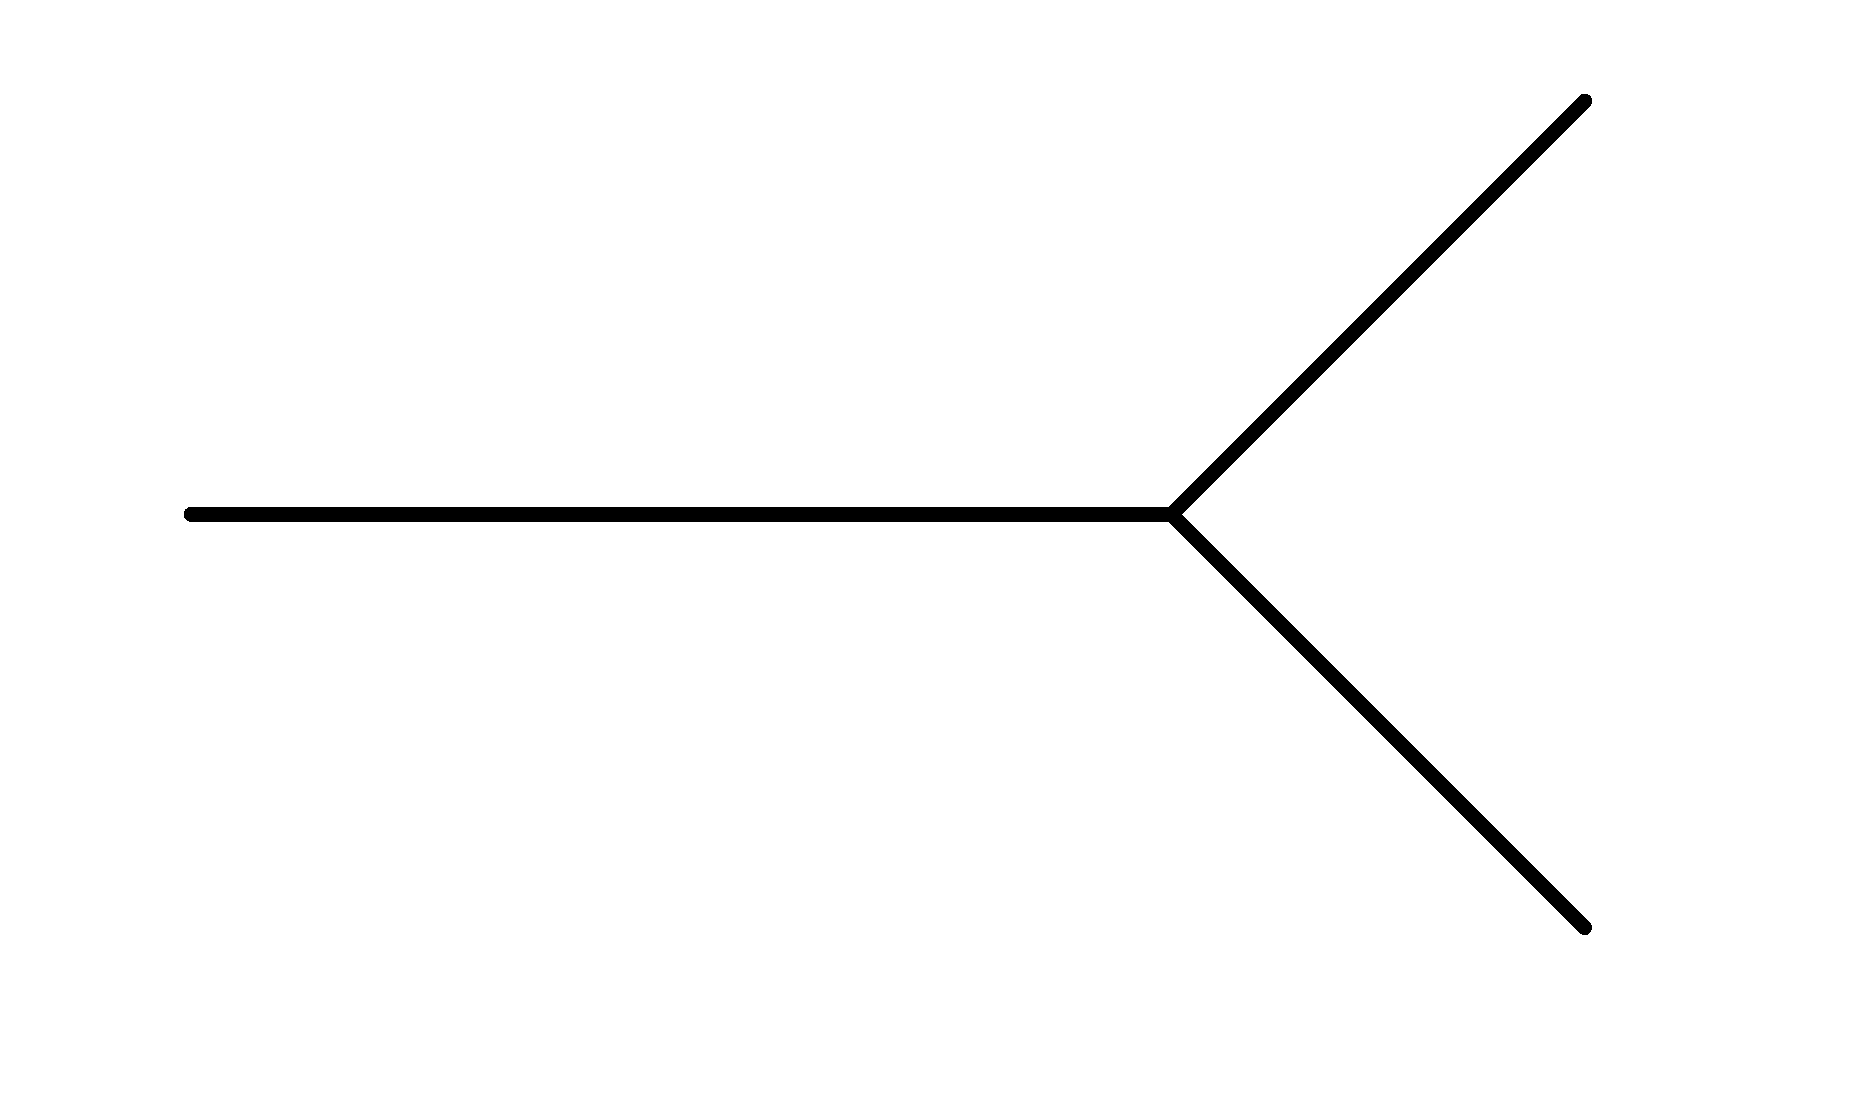
\includegraphics[scale=0.023]{./simboli/predecessor.eps}\,}



\let\oldemptyset\emptyset
\let\emptyset\varnothing
\let\o\vee
\let\e\wedge
\let\bottom\perp

\title{Applications of hyper-resolution\\{\small Abstract}}
\author{Paolo Comensoli}
\date{}

\begin{document}
 
\maketitle

\thispagestyle{empty}

In 1972 Matiyasevich published an article titled \textit{Application of the methods of the theory of logical derivation to graph theory}, in which the author successfully applies proof theoretic tools to graph theory, a field of mathematics that can appear quite far from logic. In that paper Matiyasevich gives an inductive definition of \textit{a graph which cannot be colored with n colors}. and uses it to formulate Hadwiger's conjecture and the four color theorem. 

The main proof theoretic tool used by Matiyasevich is the hyper-resolution calculus, which was developed by Robinson in 1965. In the paper \textit{A Machine-oriented logic based on the resolution principle} Robinson defines the resolution principle, a single inference principle which provides, by itself, a complete system of propositional calculus. In the following papers, he generalizes the resolution principle to hyper-resolution principle. 

In 1980 Lifschitz, starting from Matiyasevich's work, applied hyper-resolution to algebra; in particular he proved Hilbert's Nullstellensatz using Robinson's completeness theorem of hyper-resolution calculus. To achieve that proof, Lifschitz elaborated four equivalent versions of the completeness theorem; the last one is formulated in such a way that can be readily applied to many kinds of problems. In this work we will see several applications of the hyper-resolution calculus to fields of mathematics different from proof theory. 

First we will give a definition of the hyper-resolution calculus; since we are interested in applications, we will take in particular account Lifschitz's versions of the completeness theorem.
Secondly we will see applications to commutative algebra with a special focus on  Lifschitz's proof of the  Nullstellensatz. In the last chapter we will see several applications to graph theory. We will focus on coloring problems, and we will see two different ways to describe a coloring map using hyper-resolution. We will move from Matiyasevich's work,  and we will see his results using Lifschitz's versions of the completeness theorem. We will use this approach to characterize bipartite graphs and to give equivalent formulations of the four color theorem and  Hadwiger's conjecture.
\end{document}
